\smartsection{Web Server, SSL \& systemd}
\label{sec:web-server}

\smartsubsection{Overview}

This section covers the assignment's Part~1 requirements (25 points): a
C web server hosting the live dashboard, HTTPS-only access via the
self-signed certificate from Section~\ref{sec:foundation-security}, and a
systemd deployment where every service restarts automatically on failure
and starts in a well-defined dependency order.

Three systemd-managed processes make up the running system:
\begin{itemize}
    \item \texttt{surveillance-imgproc.service} --- the Python detector
    from Section~\ref{sec:image-processing}.
    \item \texttt{surveillance-web.service} --- the C dashboard server
    covered in this section.
    \item \texttt{surveillance-mqtt.service} --- the MQTT/e-mail notifier
    (Section~\ref{sec:mqtt-email}).
\end{itemize}

\smartsubsection{Web Server Architecture}

The server is a small multithreaded C program with two listeners: a plain
HTTP socket on port~80 whose only job is to 301-redirect every request to
HTTPS, and a TLS socket on port~443 serving the actual dashboard. One
detached \texttt{pthread} is spawned per HTTPS connection --- adequate for
a coursework-scale deployment (a handful of browser tabs plus
\texttt{curl} during experiments) without the complexity of an event
loop.

\begin{table}[H]
\centering
\caption{Web server source modules and their responsibilities.}
\label{tab:webserver-modules}
\resizebox{\textwidth}{!}{%
\begin{tabular}{ll}
\toprule
\textbf{Module} & \textbf{Responsibility} \\
\midrule
\texttt{main.c} & Entry point; starts the redirect thread and the HTTPS server \\
\texttt{config.c} & Parses \texttt{server.conf} (ports, cert paths, shared-memory paths) \\
\texttt{sysinfo.c} & CPU temperature, memory, CPU\% --- read directly from \texttt{/proc} and \texttt{/sys} \\
\texttt{persons\_reader.c} & Parses \texttt{persons.json} written by Section~\ref{sec:image-processing} \\
\texttt{index\_page.c} & Generates the dashboard HTML in memory \\
\texttt{mjpeg\_stream.c} & Serves \texttt{frame.jpg} as a multipart MJPEG stream \\
\texttt{redirect\_server.c} & Plain HTTP :80, 301s to the HTTPS host \\
\texttt{https\_server.c} & TLS :443; routes \texttt{/}, \texttt{/stream.mjpg}, \texttt{/stats.json} \\
\bottomrule
\end{tabular}
}
\end{table}

\keyterm{No Linux command is shelled out to at any point.} CPU temperature
comes from \texttt{/sys/class/thermal/thermal\_zone0/temp}, memory from
\texttt{/proc/meminfo}, and CPU utilization from a stateful delta between
consecutive reads of \texttt{/proc/stat}'s aggregate \texttt{cpu} line ---
satisfying the assignment's requirement that telemetry be read directly in
C.

\begin{lstlisting}[style=cstyle_bright_2026, caption={CPU utilization computed as a delta between two \texttt{/proc/stat} samples --- the first call always returns 0.0 since no prior sample exists yet, which is expected, documented behavior.}, label={code:cpu-percent}]
double sysinfo_read_cpu_percent(void) {
    static int have_prev = 0;
    static cpu_stat_t prev;
    cpu_stat_t cur;
    if (read_cpu_stat(&cur) != 0) return -1.0;
    if (!have_prev) { prev = cur; have_prev = 1; return 0.0; }
    /* ... compute (total_delta - idle_delta) / total_delta * 100 ... */
}
\end{lstlisting}

The dashboard itself embeds the live stream via a plain \texttt{<img
src="/stream.mjpg">} --- browsers render \texttt{multipart/x-mixed-replace}
natively, so no client-side video codec or JavaScript is needed for the
video path --- while a small polling loop re-fetches \texttt{/stats.json}
on a configurable interval to update the numeric readouts (person count,
CPU temperature, free memory, CPU usage).

\begin{figure}[H]
\centering
% \includegraphics[width=0.9\textwidth]{../../3.Web Server, SSL & systemd/results/fig-gitignore/webpage-demo.png}
\caption{The live dashboard: embedded MJPEG stream alongside live person count and system telemetry, refreshing automatically. \alert{Redacted before any public release} --- see the note in Section~\ref{sec:foundation-security-notes}.}\label{fig:webpage-demo}
\end{figure}

\smartsubsection{systemd Deployment}

Each service is configured with \texttt{Restart=on-failure}, and the
dependency chain is expressed with \texttt{After=}/\texttt{Requires=} so
that the web server does not start before the image-processing service is
already running:

\begin{lstlisting}[caption={\texttt{surveillance-web.service} --- dependency declaration.}, label={code:web-service-unit}]
[Unit]
After=network-online.target surveillance-imgproc.service
Wants=network-online.target
Requires=surveillance-imgproc.service

[Service]
Type=simple
User=root
Restart=on-failure
RestartSec=2
\end{lstlisting}

\texttt{surveillance-imgproc.service} additionally sets
\texttt{RestartSec=5} and 

\texttt{StartLimitIntervalSec=0}. The rationale,
specific to this project: the detector depends on the laptop's
\texttt{laptop\_stream\_webcam.sh} being reachable over the network
(Section~\ref{sec:image-processing}), and systemd's \emph{default}
restart-rate limit (five restarts within ten seconds) would otherwise
mark the service permanently \texttt{failed} if the laptop side simply
hadn't been started yet --- disabling that limit lets it retry every five
seconds indefinitely until the laptop comes online, rather than requiring
a manual \texttt{systemctl reset-failed}.

\begin{questionsection}{Why does image processing have to start before the web server?}
The assignment asks for the systemd startup ordering to be justified with
a rationale, e.g. image processing starting after camera initialization.
\end{questionsection}

\begin{answersection}{Dependency rationale}
The web server's \texttt{/stream.mjpg} and \texttt{/stats.json} endpoints
do nothing more than read whatever currently sits in
\texttt{/dev/shm/surveillance/} (Section~\ref{sec:image-processing}). If
the web server started first, it would simply serve stale or missing data
until the detector caught up --- not a crash, but a confusing, silently
wrong dashboard. Declaring \texttt{Requires=surveillance-imgproc.service}
makes this dependency explicit: systemd will not even attempt to start
the web server until the detector is confirmed running, and if the
detector later fails, \texttt{Requires=} (as opposed to the weaker
\texttt{Wants=}) means systemd also stops the web server rather than
leaving it running against a dead data source.
\end{answersection}

\smartsubsection{Experiment 1-1: Boot Time}

The initial boot-time profile showed \alert{25.697\,s} total
(3.987\,s kernel + 21.709\,s userspace) to reach
\texttt{multi-user.target}. The single largest contributor by far was
\texttt{snapd} --- \texttt{snapd.seeded.service} (11.386\,s) and
\texttt{snapd.service} (10.815\,s) together accounted for roughly 40\% of
the entire userspace boot time, on a headless board that never uses Snap
packages.

\begin{figure}[H]
\centering
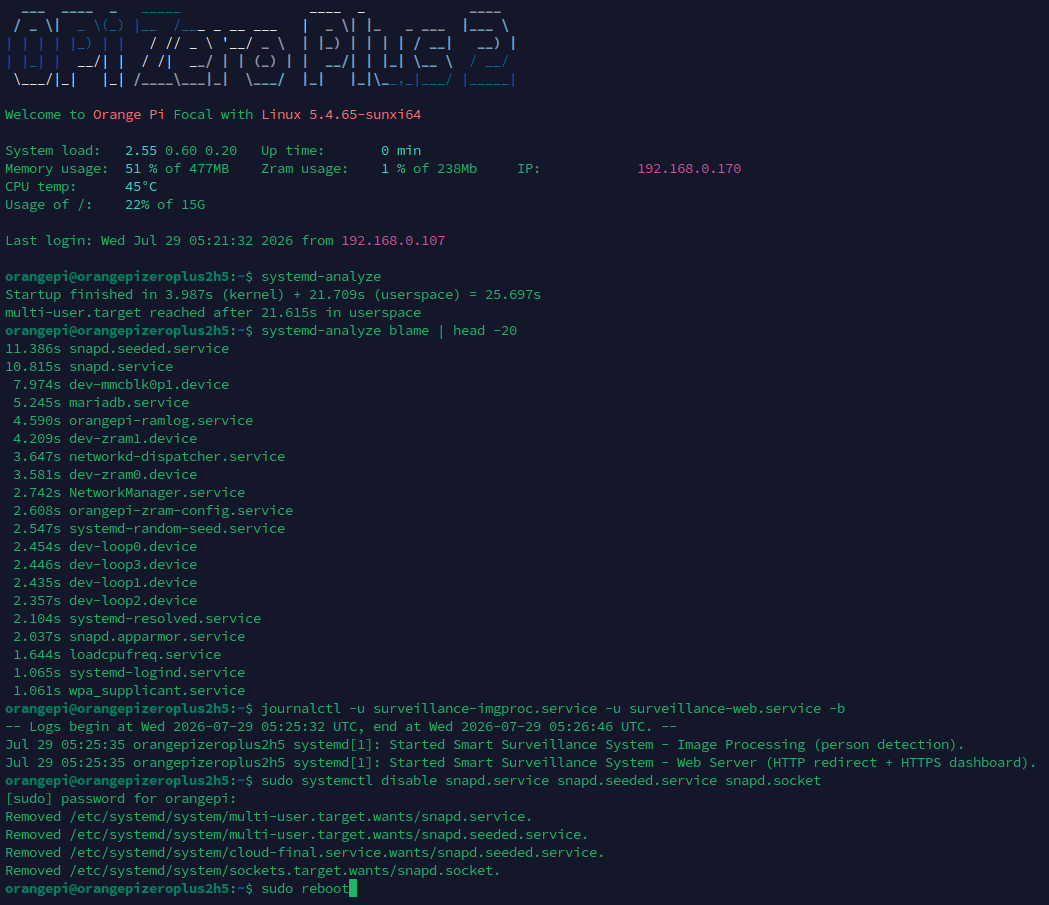
\includegraphics[width=0.95\textwidth]{../../3.Web Server, SSL & systemd/results/fig/systemd-analysis_Initial.png}
\caption{Initial boot profile: 25.697\,s total, \texttt{systemd-analyze blame} dominated by \texttt{snapd.seeded.service} and \texttt{snapd.service}.}\label{fig:systemd-initial}
\end{figure}

Two optimizations were applied: Snap was disabled entirely
(\texttt{systemctl disable snapd.service snapd.seeded.service
snapd.socket}), and the unused on-board Bluetooth service was stopped,
disabled, and masked, alongside setting the boot target explicitly to
\texttt{multi-user.target} (skipping any graphical-target resolution on a
headless board).

\begin{figure}[H]
\centering
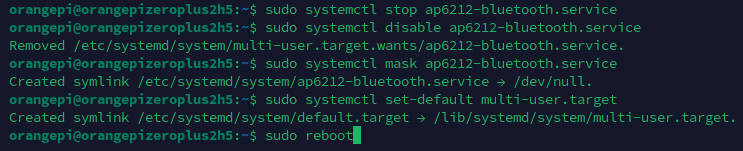
\includegraphics[width=0.85\textwidth]{../../3.Web Server, SSL & systemd/results/fig/disable-systemd-bluetooth.png}
\caption{Disabling and masking the unused \texttt{ap6212-bluetooth.service} and pinning the default target to \texttt{multi-user.target}.}\label{fig:disable-bluetooth}
\end{figure}

\begin{figure}[H]
\centering
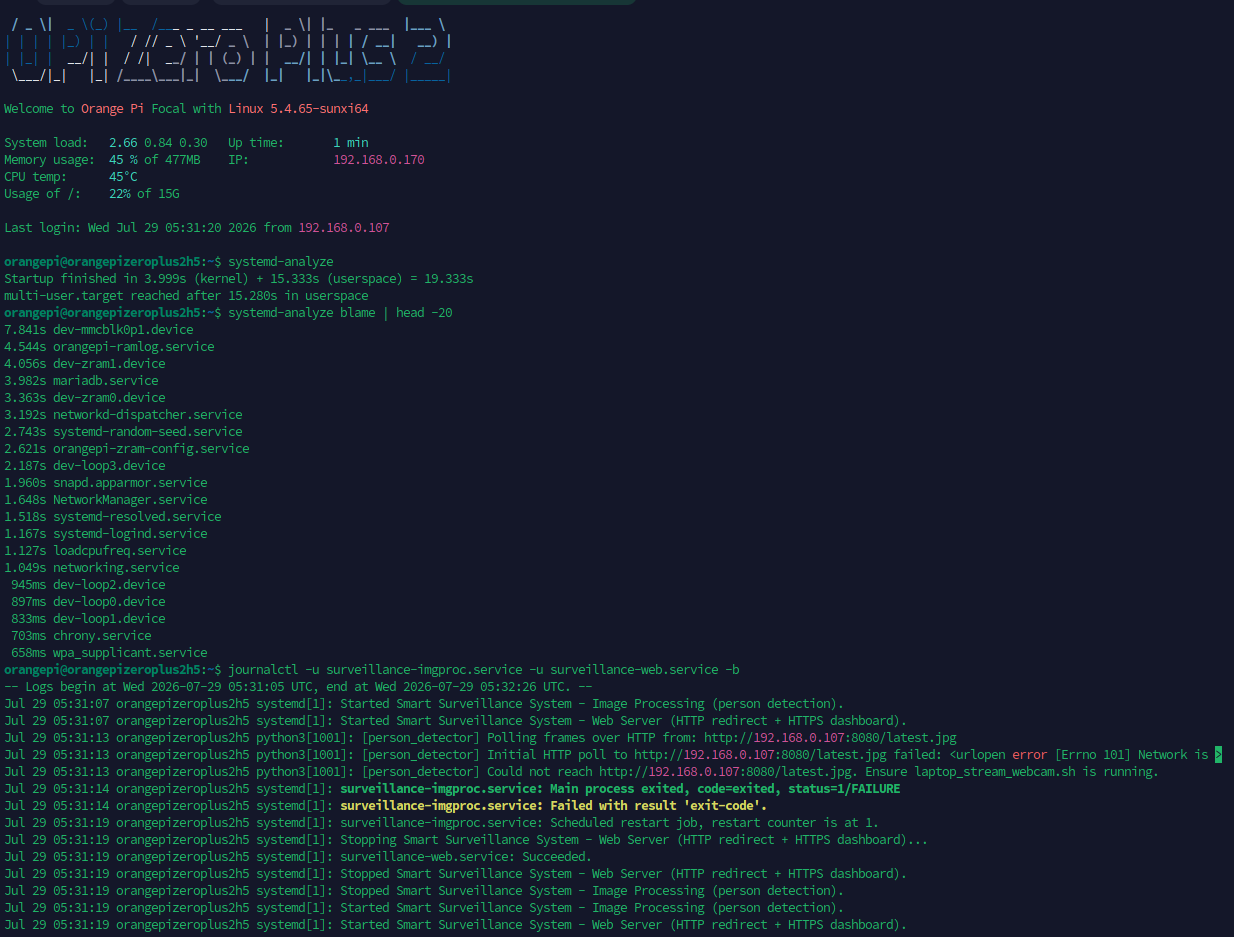
\includegraphics[width=0.95\textwidth]{../../3.Web Server, SSL & systemd/results/fig/systemd-analysis_Optimized.png}
\caption{Optimized boot profile: 19.333\,s total --- \texttt{snapd} no longer appears in the top offenders at all.}\label{fig:systemd-optimized}
\end{figure}

\begin{table}[H]
\centering
\caption{Boot time before and after removing Snap and Bluetooth.}
\label{tab:boot-time}
\begin{tabular}{lccc}
\toprule
\textbf{Configuration} & \textbf{Kernel} & \textbf{Userspace} & \textbf{Total} \\
\midrule
Initial & 3.987\,s & 21.709\,s & \alert{25.697\,s} \\
Optimized (no snapd, no Bluetooth) & 3.999\,s & 15.333\,s & \stable{19.333\,s} \\
\bottomrule
\end{tabular}
\end{table}

The optimized journalctl trace (visible at the bottom of
Figure~\ref{fig:systemd-optimized}) also captures the two application
services being started at boot in the expected order, immediately
followed by the image-processing service's HTTP-poll retry logic in
action --- \texttt{surveillance-imgproc.service} initially failing because
the laptop's webcam server was not yet reachable, then automatically
restarting per Section~\ref{sec:image-processing}'s retry design, which is
itself the intended behavior rather than a fault.

\smartsubsection{Experiment 1-2: kill -9}

The web server's main process (PID~1569) was killed with
\texttt{SIGKILL}. \texttt{systemd} detected the exit and started a
replacement process (PID~2058) automatically, with no manual intervention.

\begin{figure}[H]
\centering
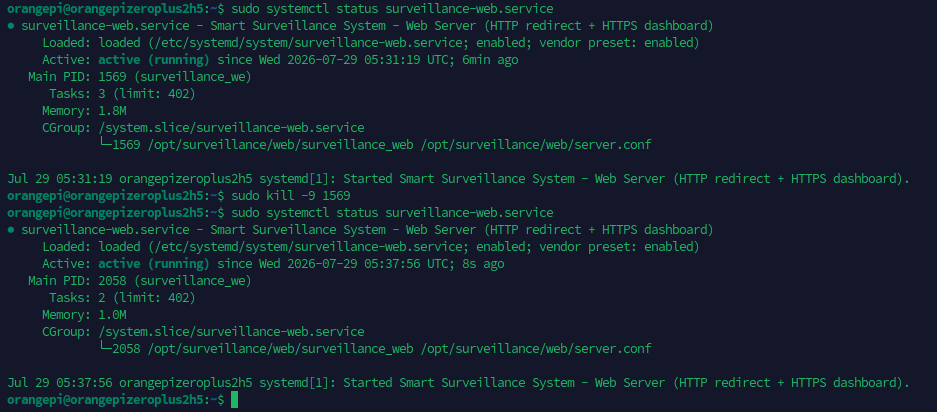
\includegraphics[width=0.95\textwidth]{../../3.Web Server, SSL & systemd/results/fig/auto-restart_webservice.png}
\caption{\texttt{sudo kill -9} against the running web server's PID, followed by \texttt{systemctl status} showing a fresh PID already active.}\label{fig:auto-restart}
\end{figure}

\smartsubsection{Experiment 1-3: Full Power Cycle}

The board was power-cycled and allowed to boot with no keyboard or mouse
attached at any point. The full boot-to-dashboard sequence was recorded
and is included as a deliverable video
(\texttt{results/video-gitignore/OrangePi\_Full-Power-Cycle\_Test.mkv})
rather than reproduced as a figure here, per the assignment's request for
a video for this specific experiment.

\smartsubsection{Experiment 1-4: HTTP to HTTPS Redirect}

A plain \texttt{curl -I} request against port~80 returns \texttt{301
Moved Permanently} with a \texttt{Location} header pointing at the HTTPS
version of the same host, confirming plaintext HTTP is never served
directly.

\begin{figure}[H]
\centering
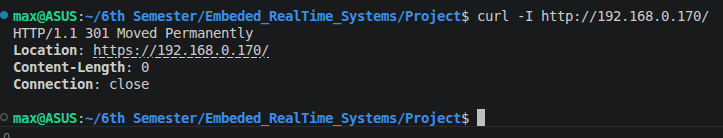
\includegraphics[width=0.75\textwidth]{../../3.Web Server, SSL & systemd/results/fig/redirect-http-to-https.png}
\caption{\texttt{curl -I http://192.168.0.170/} returning \texttt{301 Moved Permanently} with \texttt{Location: https://192.168.0.170/}.}\label{fig:redirect}
\end{figure}

\smartsubsection{Experiment 1-5: Certificate CN}

The certificate served over HTTPS was inspected in the browser's built-in
certificate viewer, confirming the Common Name field is set to the
student ID, matching the certificate generated in
Section~\ref{sec:foundation-security}.

\begin{figure}[H]
\centering
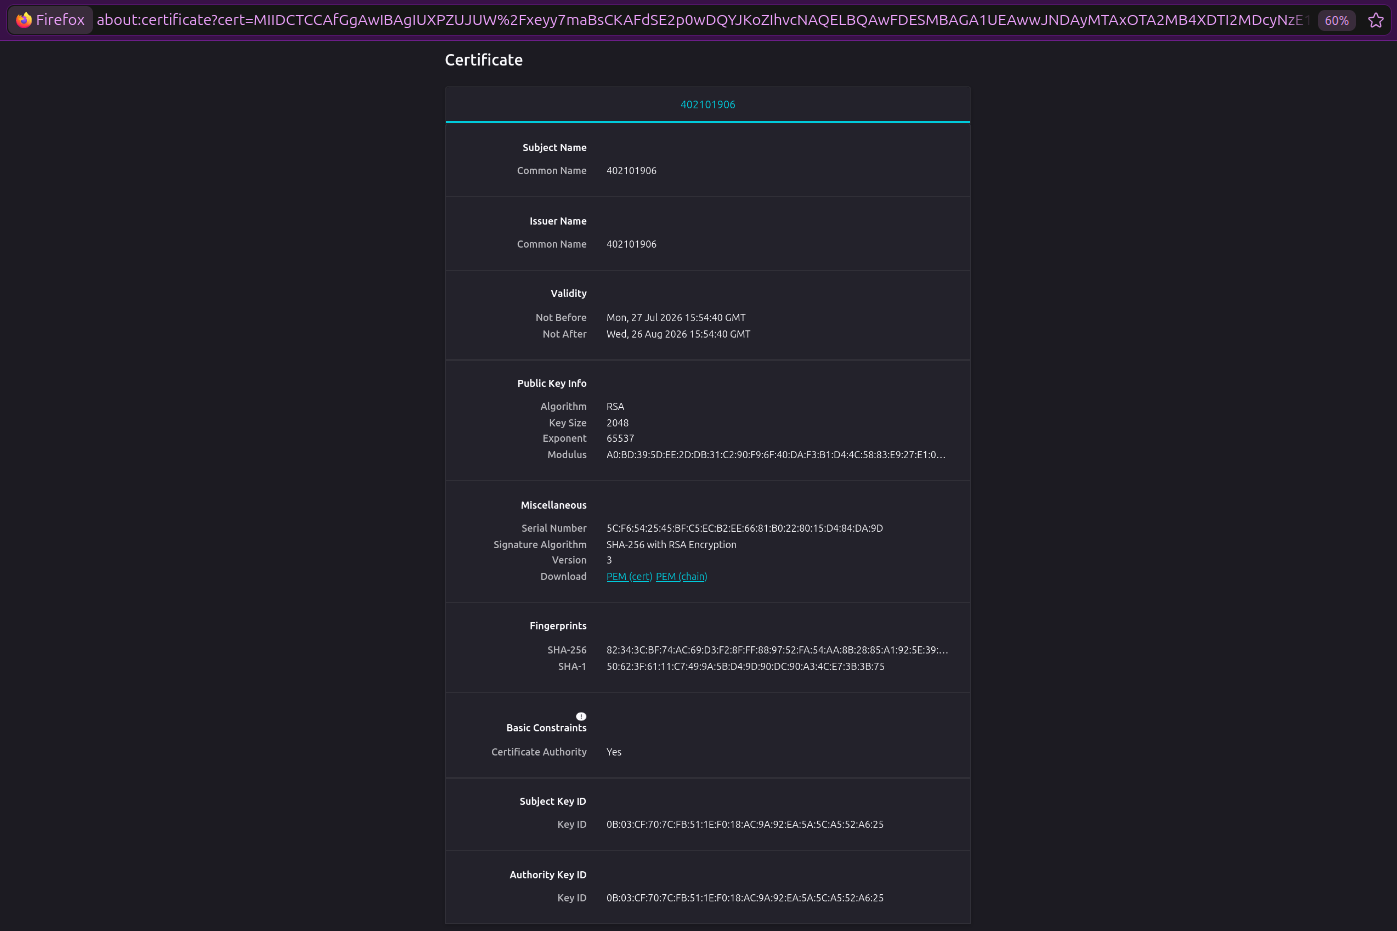
\includegraphics[width=0.85\textwidth]{../../3.Web Server, SSL & systemd/results/fig/webpage-CN-402101906.png}
\caption{Certificate viewer: Subject and Issuer Common Name \stable{402101906}, RSA 2048-bit key, 30-day validity window.}\label{fig:cert-cn}
\end{figure}

\smartsubsection{Experiment 1-6: HTML Page Shows Student ID}

The rendered dashboard's browser tab title and on-page header both
display the student's name and ID, sourced directly from
\texttt{server.conf} (see Figure~\ref{fig:webpage-demo}).

\smartsubsection{Section Summary}

\begin{table}[H]
\centering
\caption{Web Server, SSL \& systemd deliverables completed in this section.}
\label{tab:webserver-summary}
\resizebox{\textwidth}{!}{%
\begin{tabular}{ll}
\toprule
\textbf{Item} & \textbf{Status} \\
\midrule
HTML page with name + student ID in title & Complete \\
Embedded live camera stream & Complete --- MJPEG via \texttt{/stream.mjpg} \\
Live person count & Complete --- \texttt{/stats.json} \\
CPU temp / free memory / CPU usage, 2s refresh & Complete \\
HTTPS-only, self-signed cert & Complete --- CN = student ID \\
HTTP $\rightarrow$ HTTPS 301 redirect & Complete \\
systemd services, \texttt{Restart=on-failure} & Complete, all three services \\
\texttt{After=}/\texttt{Requires=} dependency chain & Complete \\
Exp.\ 1-1 (boot time) & Complete --- Table~\ref{tab:boot-time} \\
Exp.\ 1-2 (kill -9 auto-restart) & Complete \\
Exp.\ 1-3 (power cycle video) & Complete --- see video deliverable \\
Exp.\ 1-4 (HTTP redirect) & Complete \\
Exp.\ 1-5 (certificate CN) & Complete \\
Exp.\ 1-6 (page shows student ID) & Complete \\
\bottomrule
\end{tabular}%
}
\end{table}